% LaTeX2e Template by Stephen Iota (https://stepheniota.github.io/)
% last updated: Oct. 2018

% for papers
%\documentclass[aps,onecolumn,superscriptaddress]{revtex4-1}
% https://www-d0.fnal.gov/Run2Physics/WWW/templates/revtex4.pdf
% https://cdn.journals.aps.org/files/revtex/auguide4-1.pdf
% for revTeX4-1 class options

% for other
\documentclass[12pt]{article}
\usepackage[margin=2cm]{geometry}

%%%%%%%%%%%%%%%%
%%% Packages %%%
%%%%%%%%%%%%%%%%

\usepackage[utf8]{inputenc}
\usepackage{amsmath}
\usepackage{amssymb}
\usepackage{amsfonts} % to remove math font when typesetting equations
\usepackage{graphicx}
\usepackage[shortlabels]{enumitem} % to change labels in enum/item
\usepackage[dvipsnames]{xcolor} % for colored links


% always put this at the end
\usepackage[
	colorlinks=true,
	citecolor=green!50!black,
	linkcolor=NavyBlue!75!black,
	urlcolor=green!50!black,
	hypertexnames=false]{hyperref} 

 
 %%%%%%%%%%%%%%%%%%
 %% New Commands %%
 %%%%%%%%%%%%%%%%%%
 
\newcommand{\email}[1]{\texttt{\href{mailto:#1}{#1}}}

\newcommand{\hint}[1]{\color{Blue}{#1}}
 
%----------------------------------------------------
%%%%%%%%%%%%%%%%%%
%% Front Matter %%
%%%%%%%%%%%%%%%%%%

%\pagenumbering{gobble} % no page numbers
\graphicspath{{figures/}} % set directory for figures
\usepackage{wrapfig}
\setcounter{section}{-1} % start with section 0

%%%%%%%%%%%%%
%%% Title %%%
%%%%%%%%%%%%%
\begin{document}

\begin{center}

\Large{\textsc{Worksheet 7}: \textbf{Introduction to Magnetism}}

\end{center}

\vspace{.5mm}

%%%%%%%%%%
%% INFO %%
%%%%%%%%%%

\begin{tabular}{rl}
\textsc{SI Leader}:
&
Stephen Iota (\email{siota001@ucr.edu})
\\
\textsc{Course}:
&
Physics 40C (Fall 2018), Dr.~Laura Sales
\\
\textsc{Date}:
&
13 November 2018
\end{tabular}

%%%%%%%%%%%%%%
%% PROBLEMS %%
%%%%%%%%%%%%%%

\section{Review: Calculating Flux}
Find the electric flux $\Phi_E$ through surface $1$ in the figure below.
\begin{center}
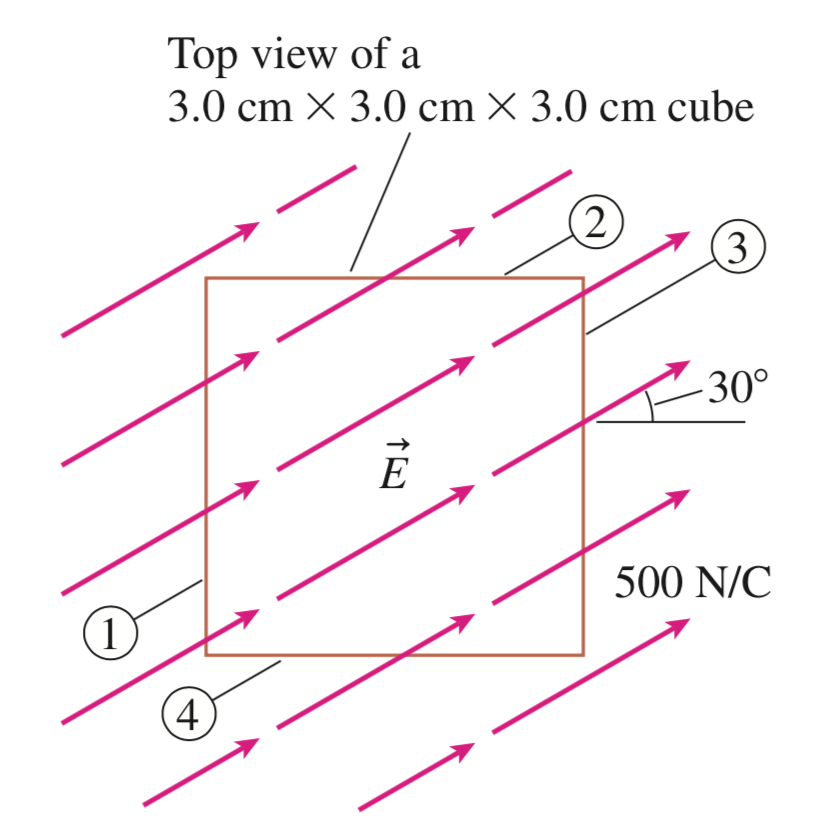
\includegraphics[width=.3\linewidth]{W7_1}		
\end{center}


\section{RHR Practice}
What is the direction of magnetic field at point $P$?

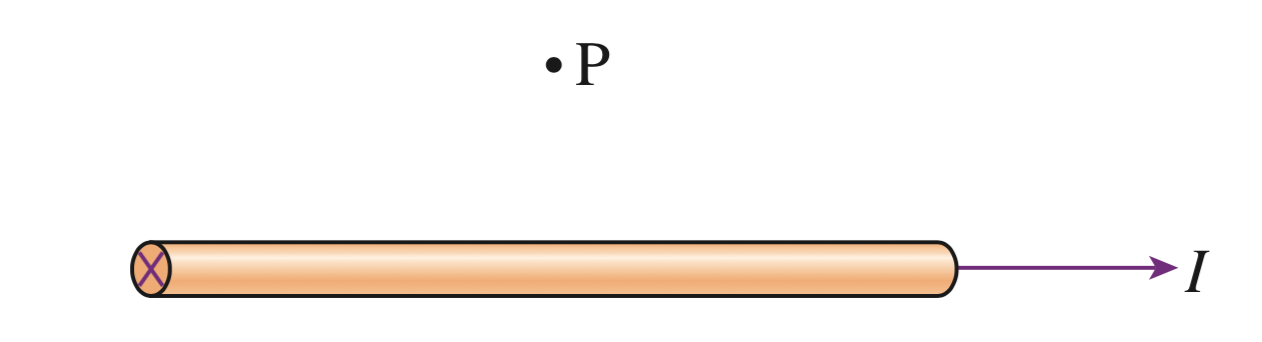
\includegraphics[width=.4\linewidth]{W7_2}

\section{Magnetic Forces between Wires}
Do the two current-carrying wires below attract or repel each other?

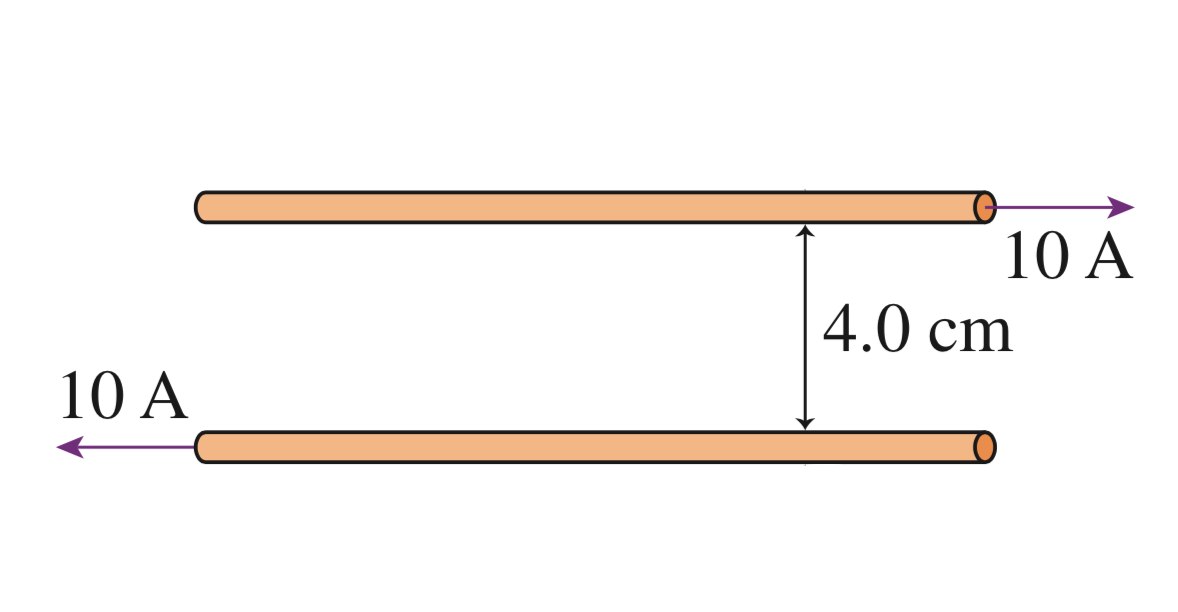
\includegraphics[width=.4\linewidth]{W7_3}

\newpage
\section{Investigating Magnetic Dipoles}

What is the current direction in the loops below?

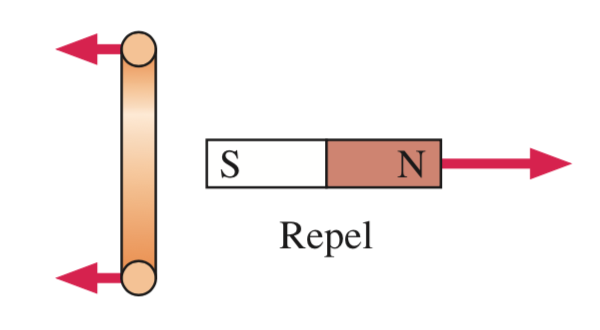
\includegraphics[width=.2\linewidth]{W7_4}

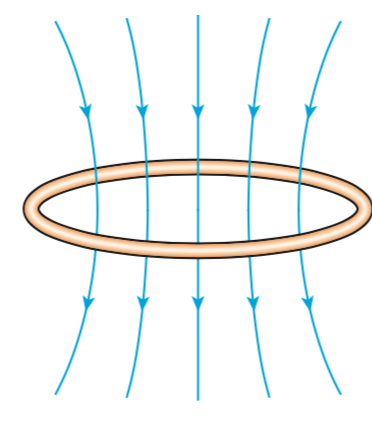
\includegraphics[width=.2\linewidth]{W7_5}



\section{Motion}

\begin{enumerate}
	\item Describe the motion of a charged particle in a magnetic field. Does velocity parallel or anti-parallel to external $\vec{B}$ field affect its trajectory?
	\item Newton's second law for circular motion is $$ F_{tan} = \frac{mv^2}{r}$$
		Find the radius of cyclotron orbit.


	
\end{enumerate}


\end{document}